\documentclass[10pt,a4paper]{report}
\addtolength{\textheight}{-2cm}
\addtolength{\textwidth}{+2cm}
%------------------------------------------------------------------------------------------------------
\usepackage{xltxtra,fontspec,xunicode}
\usepackage[slantfont,boldfont]{xeCJK} % 允许斜体和粗体

\setCJKmainfont{WenQuanYi Micro Hei}             % 缺省中文字体
\setCJKmonofont{WenQuanYi Micro Hei Mono}        % 中文等宽字体
\setmainfont{DejaVu Serif}                       % 英文衬线字体
\setsansfont{DejaVu Sans}                        % 英文无衬线字体
\setmonofont{Monaco}                             % 英文等宽字体
%-------------------------------------------------------------------------------------------------------
\linespread{1.3}                                 % 1.5倍行距,值1.6产生双倍行距
% \setlength{\parindent}{0pt}                    % 段落首行缩进
\setlength{\parskip}{1ex plus 0.5ex minus 0.2ex} % 段落间距为1ex,可让TeX在+0.5到-0.8范围内微调
                                                 % 即实际范围在0.8ex~1.5ex之间
%-------------------------------------------------------------------------------------------------------
% 页眉与页脚设置
\usepackage{fancyhdr}
\pagestyle{fancy}
\fancyhf{}                                       %清空页眉页脚
\fancyhead[LE,RO]{\thepage}                      %页眉偶数页左,奇数页右
\fancyhead[RE]{\leftmark}                        %页眉偶数页右
\fancyhead[LO]{\rightmark}                       %页眉奇数页左
% \fancyfoot[LE,RO]{\thepage}                    %页脚偶数页左,奇数页右
% \fancyfoot[RE]{\leftmark}                      %页脚偶数页右
% \fancyfoot[LO]{\rightmark}                     %页脚奇数页左
\fancypagestyle{plain}{                          %重定义plain页面样式
    \fancyhf{}
    \renewcommand{\headrulewidth}{0pt}
}
%-------------------------------------------------------------------------------------------------------
% listings 与 xcolor 配合实现源代码的语法高亮
\usepackage{xcolor}
\usepackage{listings}
\lstset{
	language=Python,
	frame = shadowbox,
	basicstyle = \ttfamily\small,
	columns = fixed,
	numbers = left,
	numberstyle = \footnotesize,
	stepnumber = 1,
	tabsize = 2,
	showspaces = false,
	showstringspaces = false,
	showtabs = false,
	captionpos = b,
	breaklines = tr[],
	breakatwhitespace = false,
	backgroundcolor = \color{white},
	keywordstyle=\color{blue},
	numberstyle=\color[RGB]{0,192,192},
	commentstyle=\color[RGB]{0,96,96},
	stringstyle=\ttfamily\slshape\color[RGB]{128,0,0},
	escapeinside=``
}
%-------------------------------------------------------------------------------------------------------
\usepackage{graphicx}                            % 引入图片
\graphicspath{{img/}{images/}}                   % 要导入的图片的位置。可以有多个目录,但就算只有一个目录,也要用两级花括号
%-------------------------------------------------------------------------------------------------------
	\title{文章标题}                             % 文章的标题
	\author{                                     % 作者与致谢
		阿左 \thanks{感谢读者} \and 
		Nobody \thanks{感谢国家}
	}
	\date{\today}                                % 日期
	
%-------------------------------------------------------------------------------------------------------
\begin{document}
	\maketitle                                   % 制作标题
	\tableofcontents                             % 生成章节目录
	\setcounter{tocdepth}{5}                     % 生成章节的目录深度
	\listoffigures                               % 生成图片目录
	\listoftables                                % 生成表格目录


%	\begin{abstract}                             % 英文摘要
%		this is for english abstract
%	\end{abstract}
%
%	\renewcommand{\abstractname}{摘要}           % 中文摘要
%	\begin{abstract}
%		这里是摘要的内容
%	\end{abstract}

	\part{语法基础}

		\chapter{OOP与类}
	
	在python中,同一个模块只能有一个实例,当一个模块的代码被修改以后必须重新加载模块才能生效;而是python中的一个类可以同时创建多个实例(即对象)。

	python中把数据保存在对象中,相关的操作(方法)在类中。

	\section{Python基本类概念}

		\subsection{类的继承}
 			\lstinputlisting[label=ch12:subclass, caption=类继承]{py/expoo01.py}

		\subsection{类的属性与方法}
			对于类和对象,无论属性还是方法。python都作为变量处理。
			\lstinputlisting[label=ch12:funcandattr, caption=类的属性与方法]{py/expoop002.py}


% \chapter{基本使用}
% 
% 	\section{常用的格式}
% 
% 		\subsection{基本的段落}
% 			空行可以自然分隔段落:
% 
% 			可以设定字体为\textit{斜体};给文字加上\underline{下划线}。可以设定字体为\textit{斜体};给文字加上\underline{下划线}。可以设定字体为\textit{斜体};给文字加上\underline{下划线}。可以设定字体为\textit{斜体};给文字加上\underline{下划线}。
% 
% 			可以设定字体为\textit{斜体};给文字加上\underline{下划线}。可以设定字体为\textit{斜体};给文字加上\underline{下划线}。可以设定字体为\textit{斜体};给文字加上\underline{下划线}。可以设定字体为\textit{斜体};给文字加上\underline{下划线}。
% 
% 			可以设定字体为\textit{斜体};给文字加上\underline{下划线}。可以设定字体为\textit{斜体};给文字加上\underline{下划线}。可以设定字体为\textit{斜体};给文字加上\underline{下划线}。可以设定字体为\textit{斜体};给文字加上\underline{下划线}。
% 
% 		\subsection{边注与脚注}
% 			按照国际惯例,这里是鬼扯的部分。\footnote{我才不承认这是为了骗稿费呢~}
% 
% 			同样也给内容加上连注。但边注是没有编号的,因为就在旁边。\marginpar{这里是边注的内容。}
% 
% 		\subsection{原文照排}
% 			在正文中放入源文照排:在Linux下通过\verb|ls -al|查看当前目录下所有文件。
% 
% 			多行的原文照排要用到verbatim环境:
% 			\begin{verbatim}
% 				/* 输出10行"Hello, world!"的面试题 */
% 				/* 某位童鞋的答案是这样写的        */
% 				printf("Hello, world!");
% 				printf("Hello, world!");
% 				printf("Hello, world!");
% 				printf("Hello, world!");
% 				printf("Hello, world!");
% 				printf("Hello, world!");
% 				printf("Hello, world!");
% 				printf("Hello, world!");
% 				printf("Hello, world!");
% 				printf("Hello, world!");
% 			\end{verbatim}
% 
% 			原文照排时强调空格到verbatim*环境:
% 			\begin{verbatim*}
% 				printf("Hello, world!");
% 			\end{verbatim*}
% 
% 		\subsection{程序代码}
% 
% 			使用listings宏包的效果:
% 
% \begin{lstlisting}[language=C]
% #include <stdio.h>
% 
% int main(int argc, char ** argv)
% {
% 	printf("Hello world!\n");
% 	/** 看起来直接用listings和xelatex配合显示中文没有问题 **/
% 	printf("显示中文!\n");
% 	return 0;
% }
% \end{lstlisting}
% 
% 			可以只引用整个代码中的一部分:
% 
% \begin{lstlisting}[language=C,firstline=3,lastline=9]
% #include <stdio.h>
% 
% int main(int argc, char ** argv)
% {
% 	printf("Hello world!\n");
% 	/** 看起来直接用listings和xelatex配合显示中文没有问题s1l1O0O0 **/
% 	printf("显示中文!\n");
% 	return 0;
% }
% \end{lstlisting}
% 
% 			使用\verb|\lstinputlisting|引用外部文件:
% 
% 			\lstinputlisting[language=HTML,firstline=2,lastline=8]{src/aa.html}
% 
% 	\section{图片与表格}
% 
% 		\subsection{使用图片}
% 
% 			试试使用浮动环境插入图片,但是这样图片就不知道浮动到什么地方去了:
% 
% 			\begin{figure}[htbp]                        % 
% 				\centering                              % 图片居中	
% 				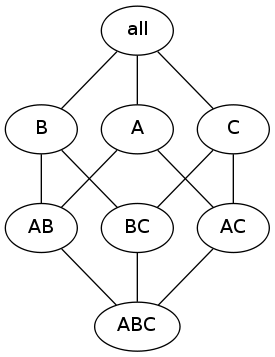
\includegraphics[scale=0.5]{dm0201.png} % scale指定缩放
% 				\caption{第一张浮动的图片}            % 图片的标题,会自动编号
% 				\label{dm0201}                % 图片的标记,一定要加在caption后面。不然指向的是前一个插图
% 			\end{figure}
% 
% 			试试使用浮动环境插入图片,但是这样图片就不知道浮动到什么地方去了:
% 
% 			\begin{figure}[htbp]                        % 
% 				\centering                              % 图片居中	
% 				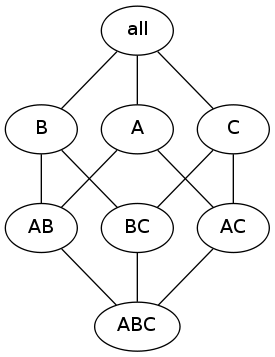
\includegraphics[scale=0.5]{dm0201.png} % scale指定缩放
% 				\caption{第二张浮动的图片}            % 图片的标题,会自动编号
% 				\label{dm0202}                % 图片的标记,一定要加在caption后面。不然指向的是前一个插图
% 			\end{figure}
% 
% 			试试使用浮动环境插入图片,但是这样图片就不知道浮动到什么地方去了:
% 
% 			\begin{figure}[htbp]                        % 
% 				\centering                              % 图片居中	
% 				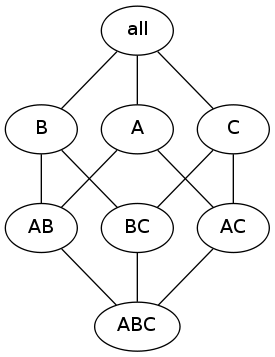
\includegraphics[scale=0.5]{dm0201.png} % scale指定缩放
% 				\caption{第三张浮动的图片}            % 图片的标题,会自动编号
% 				\label{dm0203}                % 图片的标记,一定要加在caption后面。不然指向的是前一个插图
% 			\end{figure}
% 
% 		\subsection{使用表格}
% 
% 			组表格也加上浮动环境:
% 
% 			\begin{table}[htbp]
% 				\caption{浮动环境中的三线表}
% 				\label{tab:threesome}
% 				\centering
% 				\begin{tabular}{lll}
% 					\hline
% 					操作系统 & 发行版 & 编辑器 \\
% 					\hline
% 					Windows & MikTeX & TeXnicCenter \\
% 					Unix/Linux & TeX Live & Emacs \\
% 					Mac OS & MacTeX & TeXShop \\
% 					\hline
% 				\end{tabular}
% 			\end{table}
% 

\end{document}
